%!TEX root = ../thesis.tex
%*******************************************************************************
%****************************** Third Chapter **********************************
%*******************************************************************************
\chapter{Results and Discussion}

% **************************** Define Graphics Path **************************
\ifpdf
    \graphicspath{{Chapter3/Figs/Raster/}{Chapter3/Figs/PDF/}{Chapter3/Figs/}}
\else
    \graphicspath{{Chapter3/Figs/Vector/}{Chapter3/Figs/}}
\fi

In this chapter we present the performance of the classifiers under the different split schemes outlined earlier. The various features used and their applicability on different splitting conditions is also be evaluated. 

The confusion matrix used has the form 
\begin{align}
	\begin{bmatrix}
	\text{True Black/ Black Predicted correctly}&\text{False White/ Black  Predicted falsely}\\
	\text{False Black/ White Predicted falsely}&\text{True White/ White  Predicted correctly}
	\end{bmatrix}
\end{align}



The results of the benchmark method we devised in section \ref{sec:splitting} are presented in table \ref{table:benchmarksim} for maximum similarity, table \ref{table:benchmarkdissim} for maximum dissimilarity, and table \ref{table:benchmarkrand} for random splits. The two row names differentiate between the set of response variables used for the benchmark's evaluation; All Labels indicates the use of all the river samples, Min Labels of those whose total OTU read-count is more than 10000. The accuracy is also included in a separate row so as to make comparisons between methods easier. A quick glance shows that the benchmark has a much lower accuracy than the class prior of the data set (87.2\%), as was suggested in section \ref{sec:splitting}.



\begin{table}
	\centering
	\begin{tabular}{l c c c}
		\toprule 
		&\multicolumn{2}{c}{Confusion Matrix} &Accuracy\\
		Features used & Predicted Black&Predicted White&\\ 
		
		\midrule
		\multirow{2}{*}{All Labels }& 	2.64 & 18.36&		\multirow{2}{*}{77.6\%}\\
					&	18.36 &124.64&\\
		\cmidrule{2-3}
		\multirow{2}{*}{Min Labels}  &2.75 & 18.25&		\multirow{2}{*}{76.8\%}\\
		&18.25& 117.75&\\
		\bottomrule

	\end{tabular}
	\caption{Benchmark for Maximum Similarity}
	\label{table:benchmarksim}
\end{table}

\begin{table}[h]
	\centering
	\begin{tabular}{l c c c }
		\toprule 
		&\multicolumn{2}{c}{Confusion Matrix} & Accuracy\\
		Features used & Predicted Black&Predicted White&\\ 
		
		\midrule
		\multirow{2}{*}{All Labels }&  1.75 &19.25&\multirow{2}{*}{76.7\%}\\
								  &	 18.96&124.04 &\\
		\cmidrule{2-3}
		\multirow{2}{*}{Min Labels}    &1.83&19.17&\multirow{2}{*}{75.8\% }\\
									&18.83&117.17&\\
		\bottomrule

	\end{tabular}
	\caption{Benchmark for Maximum Dissimilarity}
	\label{table:benchmarkdissim}
\end{table}

%RANDOM SPLITS
\begin{table}[h]
	\centering
	\begin{tabular}{l c c c }
		\toprule 
		&\multicolumn{2}{c}{Confusion Matrix} & Accuracy\\
		Features used & Predicted Black&Predicted White&\\ 
		
		\midrule
		\multirow{2}{*}{All Labels }& 2.69 &18.31&\multirow{2}{*}{77.7\%}\\
		&	 18.31&124.69 &\\
		\cmidrule{2-3}
		\multirow{2}{*}{Min Labels}    &2.81&18.19&\multirow{2}{*}{76.8\% }\\
		&18.19&117.81&\\
		\bottomrule
	\end{tabular}
	\caption{Benchmark for Maximum Dissimilarity}
	\label{table:benchmarkrand}
\end{table}
%%%
%
%SIMILARITY
\section{Maximum Similarity}
The results for Logistic regression and Random forest tested on the maximum similarity scheme are shown in tables \ref{table:lrdissimilarity} and \ref{table:rfrsimilarity} respectively. Both methods performed relatively well when compared to the baseline. Furthermore, the PCoA features produced poorer results than the OTU ones. This was also the case when fewer dimensions, describing 99\% and 90\% of the variance, were chosen as features. The results for these can be found in the appendix.

Using the F score to find the best model in the cross validation step resulted in a lower number of black water samples correctly identified. This was especially the case of Random Forest. Therefore, we present the performance of the models selected using accuracy.

Just from the accuracy score we can see that Logistic regression outperforms Random Forests. The best score for the former is 98.78\% using OTU LOW and close second is 98.17\% using OTU, OTU CSS, and OTU CSS LOG. For Random Forests, OTU CSS LOG has the best score of 96.95\% and close second is OTU CSS and OTU LOW with 96.34\%. Both methods have significantly better results than the baseline's 77.6\% and 76.8\% accuracy (the second is used to compare the OTU MIN CSS set).

Using the $L_1$ penalty in Logistic regression has reduced the coefficients of many features to zero. From the best performing sets, the percentage of zero coefficients to the total number is 82.34\% (OTU LOW), 85.29\% (OTU), 88.95\% (OTU CSS), and 95.32\% (OTU CSS LOG). From the remaining species, 3.79\% of them have non zero coefficients in three sets (OTU CSS< OTU CSS LOG, and OTU). This means that there are only a limited number of informative species that help us identify the water colour. 


%LOGISTIC SIM
\begin{table}[h]
\centering
\begin{tabular}{l c  c c}
\toprule
		&\multicolumn{2}{c}{Confusion Matrix} & Accuracy\\
Features used & Predicted Black&Predicted White&\\
\midrule
\multirow{2}{*}{OTU} &19 &2&\multirow{2}{*}{98.17\%}\\
&	 1&142&\\
\cmidrule{2-3}
\multirow{2}{*}{OTU LOW} &19 &2&\multirow{2}{*}{98.78\%}\\
&	 0&143&\\
\cmidrule{2-3}
\multirow{2}{*}{OTU CSS}&18 &3&\multirow{2}{*}{98.17\%}\\
&	 0&143&\\
\cmidrule{2-3}
\multirow{2}{*}{OTU Min CSS}&18 &3&\multirow{2}{*}{98.09\%}\\
&	 0&136&\\
\cmidrule{2-3}
\multirow{2}{*}{OTU CSS LOG}&19 &2&\multirow{2}{*}{98.17\%}\\
&	 1&142&\\
\cmidrule{2-3}
\multirow{2}{*}{PCoA Bray-Curtis} &16 &5&\multirow{2}{*}{95.12\%}\\
&	 3&140&\\
\cmidrule{2-3}
\multirow{2}{*}{PCoA Bray-Curtis CSS} &16 &5&\multirow{2}{*}{96.34\%}\\
&	 1&142&\\
\bottomrule
\end{tabular}
\caption{Results from maximising similarity using Logistic Regression}
\label{table:lrsimilarity}
\end{table}


% RFR similarirtty
\begin{table}[h]
	\centering
\begin{tabular}{l c  c c}
	\toprule
	&\multicolumn{2}{c}{Confusion Matrix} & Accuracy\\
	Features used & Predicted Black&Predicted White&\\
	
	\midrule
	\multirow{2}{*}{OTU} &17 &4&\multirow{2}{*}{95.73\%}\\
	&	 3&140&\\
	\cmidrule{2-3}
	\multirow{2}{*}{OTU LOW} &18 &3&\multirow{2}{*}{96.34\%}\\
	&	 3&140&\\
	\cmidrule{2-3}
	\multirow{2}{*}{OTU CSS} &18 &3&\multirow{2}{*}{96.34\%}\\
	&	 3&140&\\
	\cmidrule{2-3}
	\multirow{2}{*}{OTU Min CSS}&18 &3&\multirow{2}{*}{96.18\%}\\
	&	 3&133&\\
	\cmidrule{2-3}
	\multirow{2}{*}{OTU CSS LOG} &19 &2&\multirow{2}{*}{96.95\%}\\
	&	 3&140&\\
	\cmidrule{2-3}
	\multirow{2}{*}{PCoA Bray-Curtis} &6 &15&\multirow{2}{*}{88.41\%}\\
	&	 4&139&\\
	\cmidrule{2-3}
	\multirow{2}{*}{PCoA Bray-Curtis CSS} &4 &17&\multirow{2}{*}{89.63\%}\\
	&	 0&143&\\
	\bottomrule
\end{tabular}
\caption{Results from maximising similarity using Random Forest}
\label{table:rfrsimilarity}
\end{table}

To explore which of these species contribute most to classification we used the feature importance of Random Forests. However, instead of checking only for individual species' predictive ability, we used the taxonomic order as an aggregating factor, to get a sense which contributes the most. This was done by averaging the importance of each species, as reported by Random Forests, within their Order. The results are presented for some feature sets in the form of pie charts in Figures \ref{fig:simmeanotucss} and \ref{fig:simmeanotucsslog}. 

For all feature sets used, species in the \textit{Perissodactyla} Order have on average the most explanatory power. However, this Order is only composed of two (sub)species; the South American and Mountain tapir. This method of aggregating feature importance thus favours orders with few species. It is evident in the next most important taxonomic Order as well, the \textit{Caticea}, which is again composed of two species; the Amazon river dolphin (which is technically a whale) and Tucuxi (a freshwater dolphin). 

Therefore, another aggregating method has to be used to get a better idea of the explanatory power of the whole taxonomic Order. We chose to do this by summing the importance of each species, within their Order. The results are shown in Figures \ref{fig:simsumotucss} and \ref{fig:simsumotucsslog}, and highlight different Order. In particular, \textit{Characiformes }and \textit{Siluriformes} are in sum the most explanatory ones. This is to be expected however, since they are the most populous as well (although in reverse order) and summing importance will inevitably favour the most numerous groups. 



\begin{figure}[h]
	\centering

	\begin{subfigure}{0.45\textwidth}
	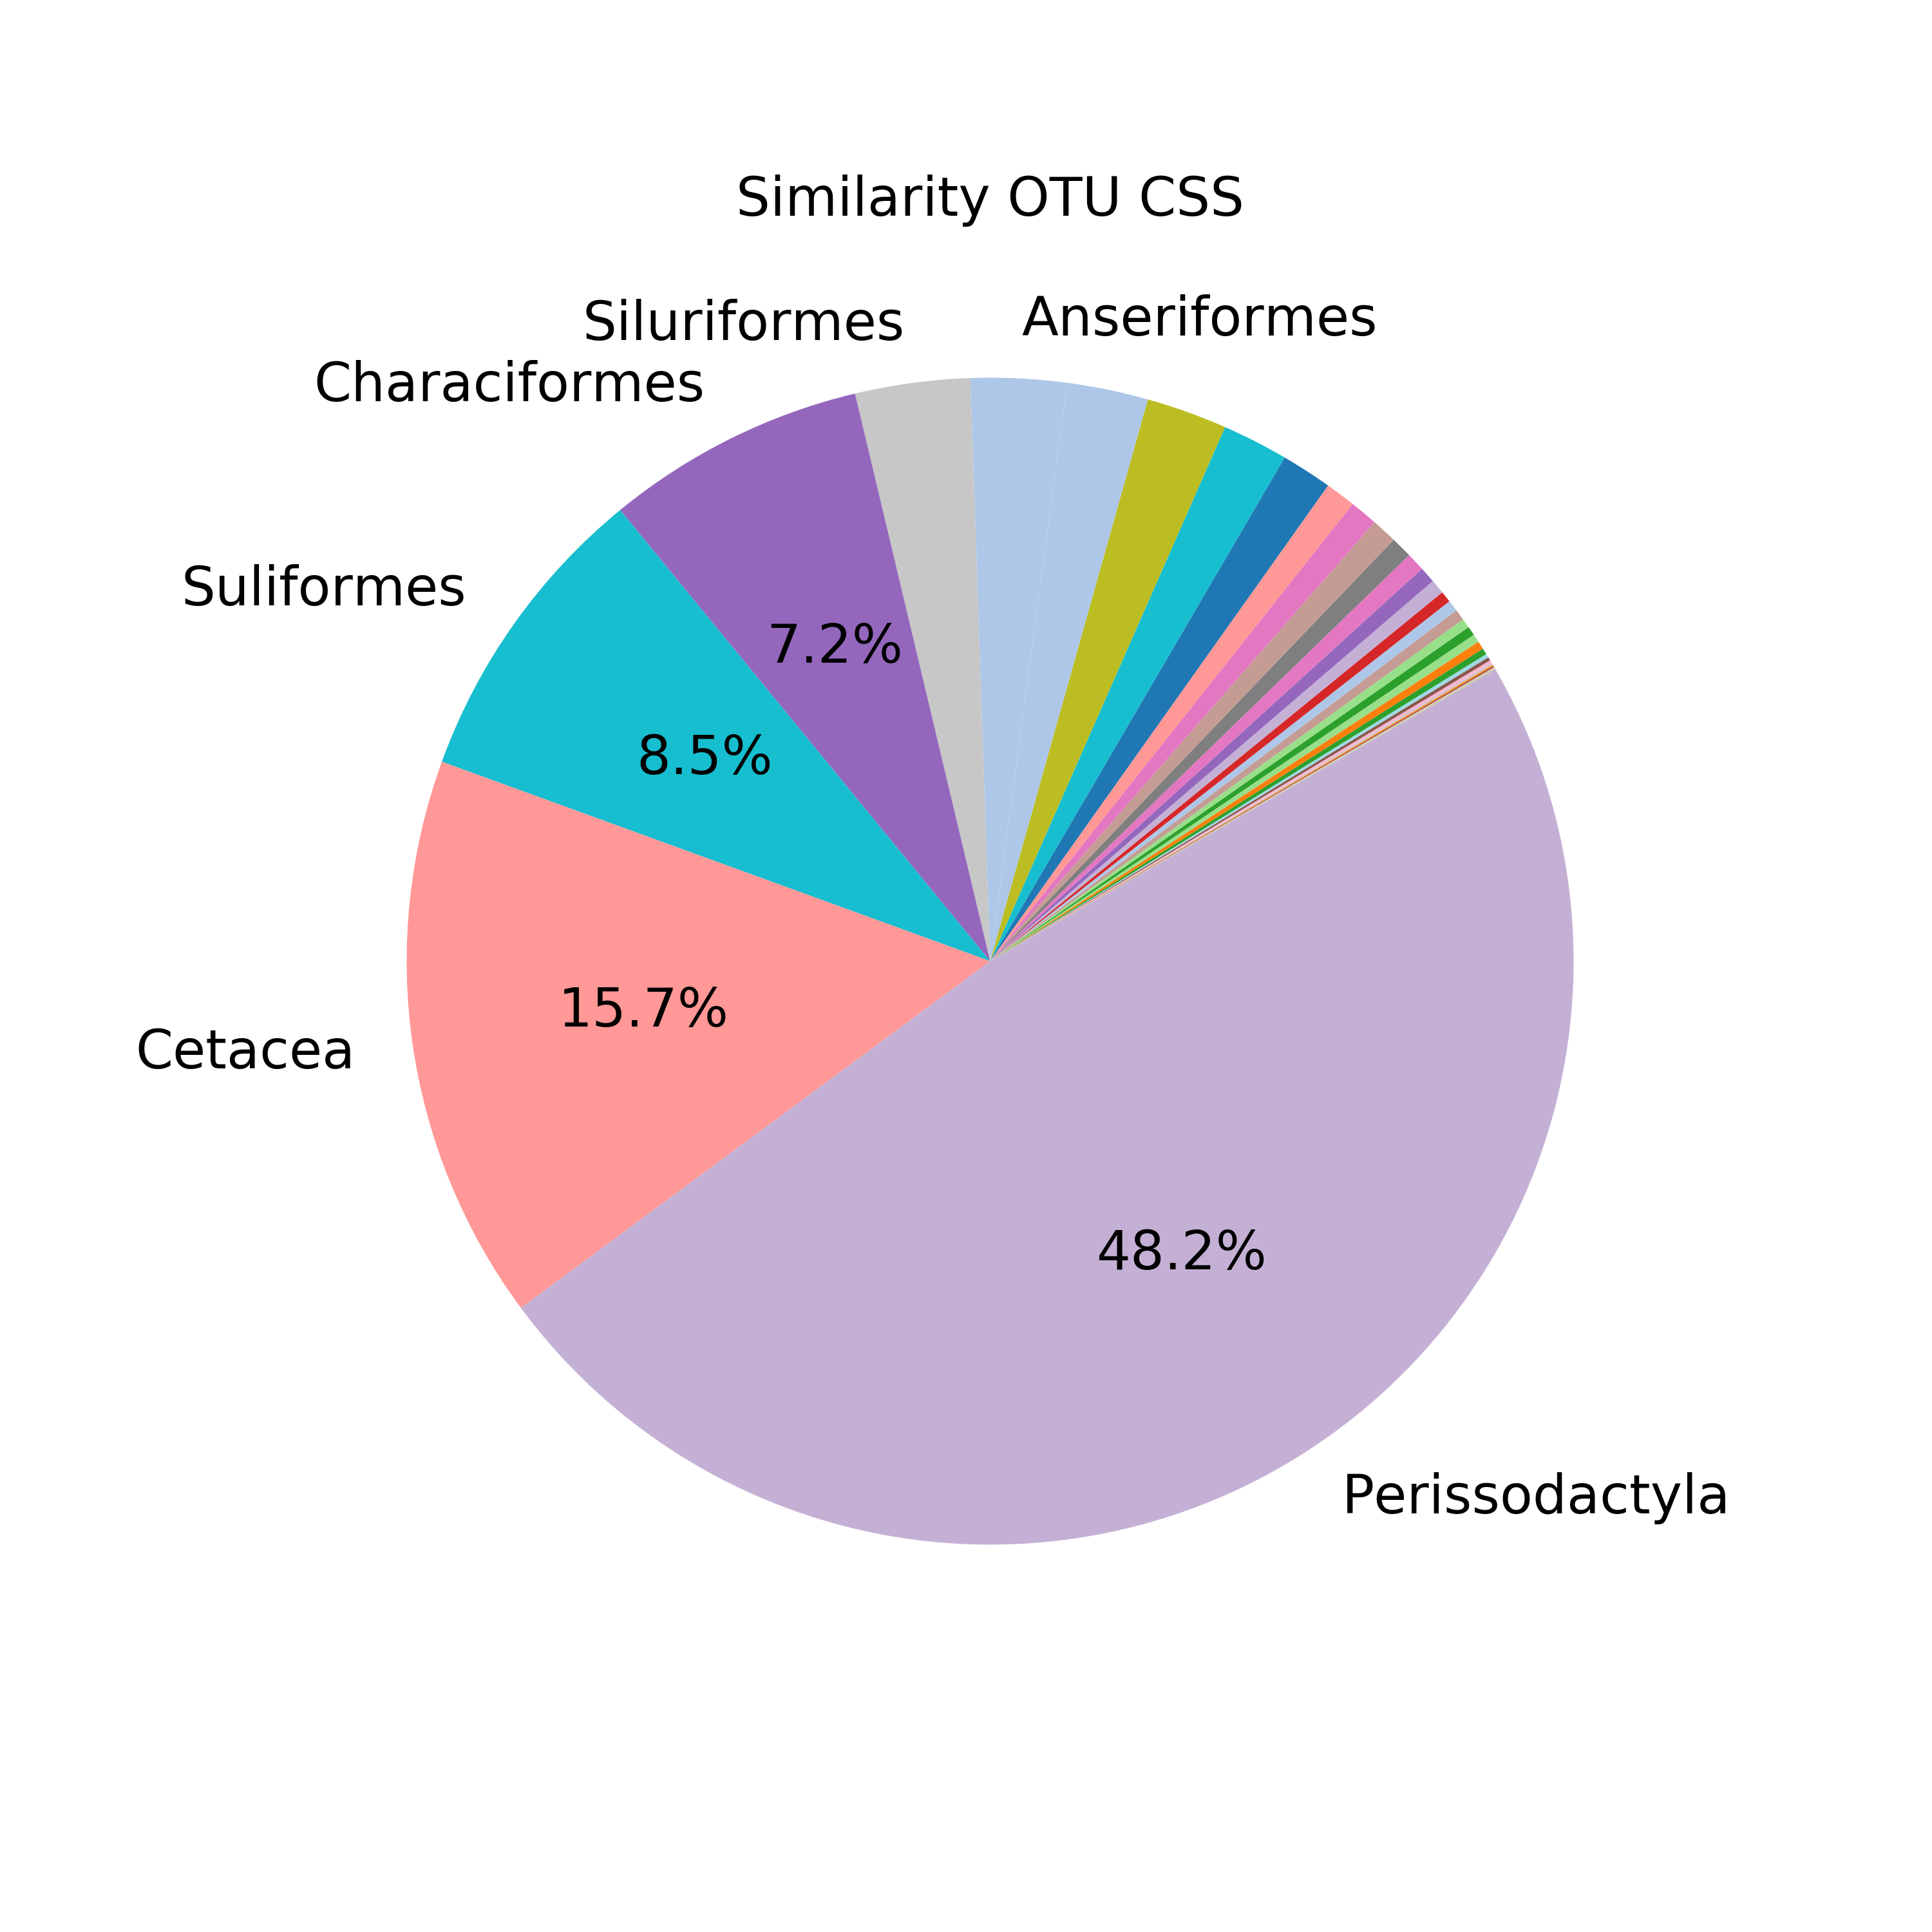
\includegraphics[width=\textwidth]{rfr_sim_mean_pieOTU CSS}
	\caption{}
	\label{fig:simmeanotucss}
	\end{subfigure}	
	\begin{subfigure}{0.45\textwidth}
		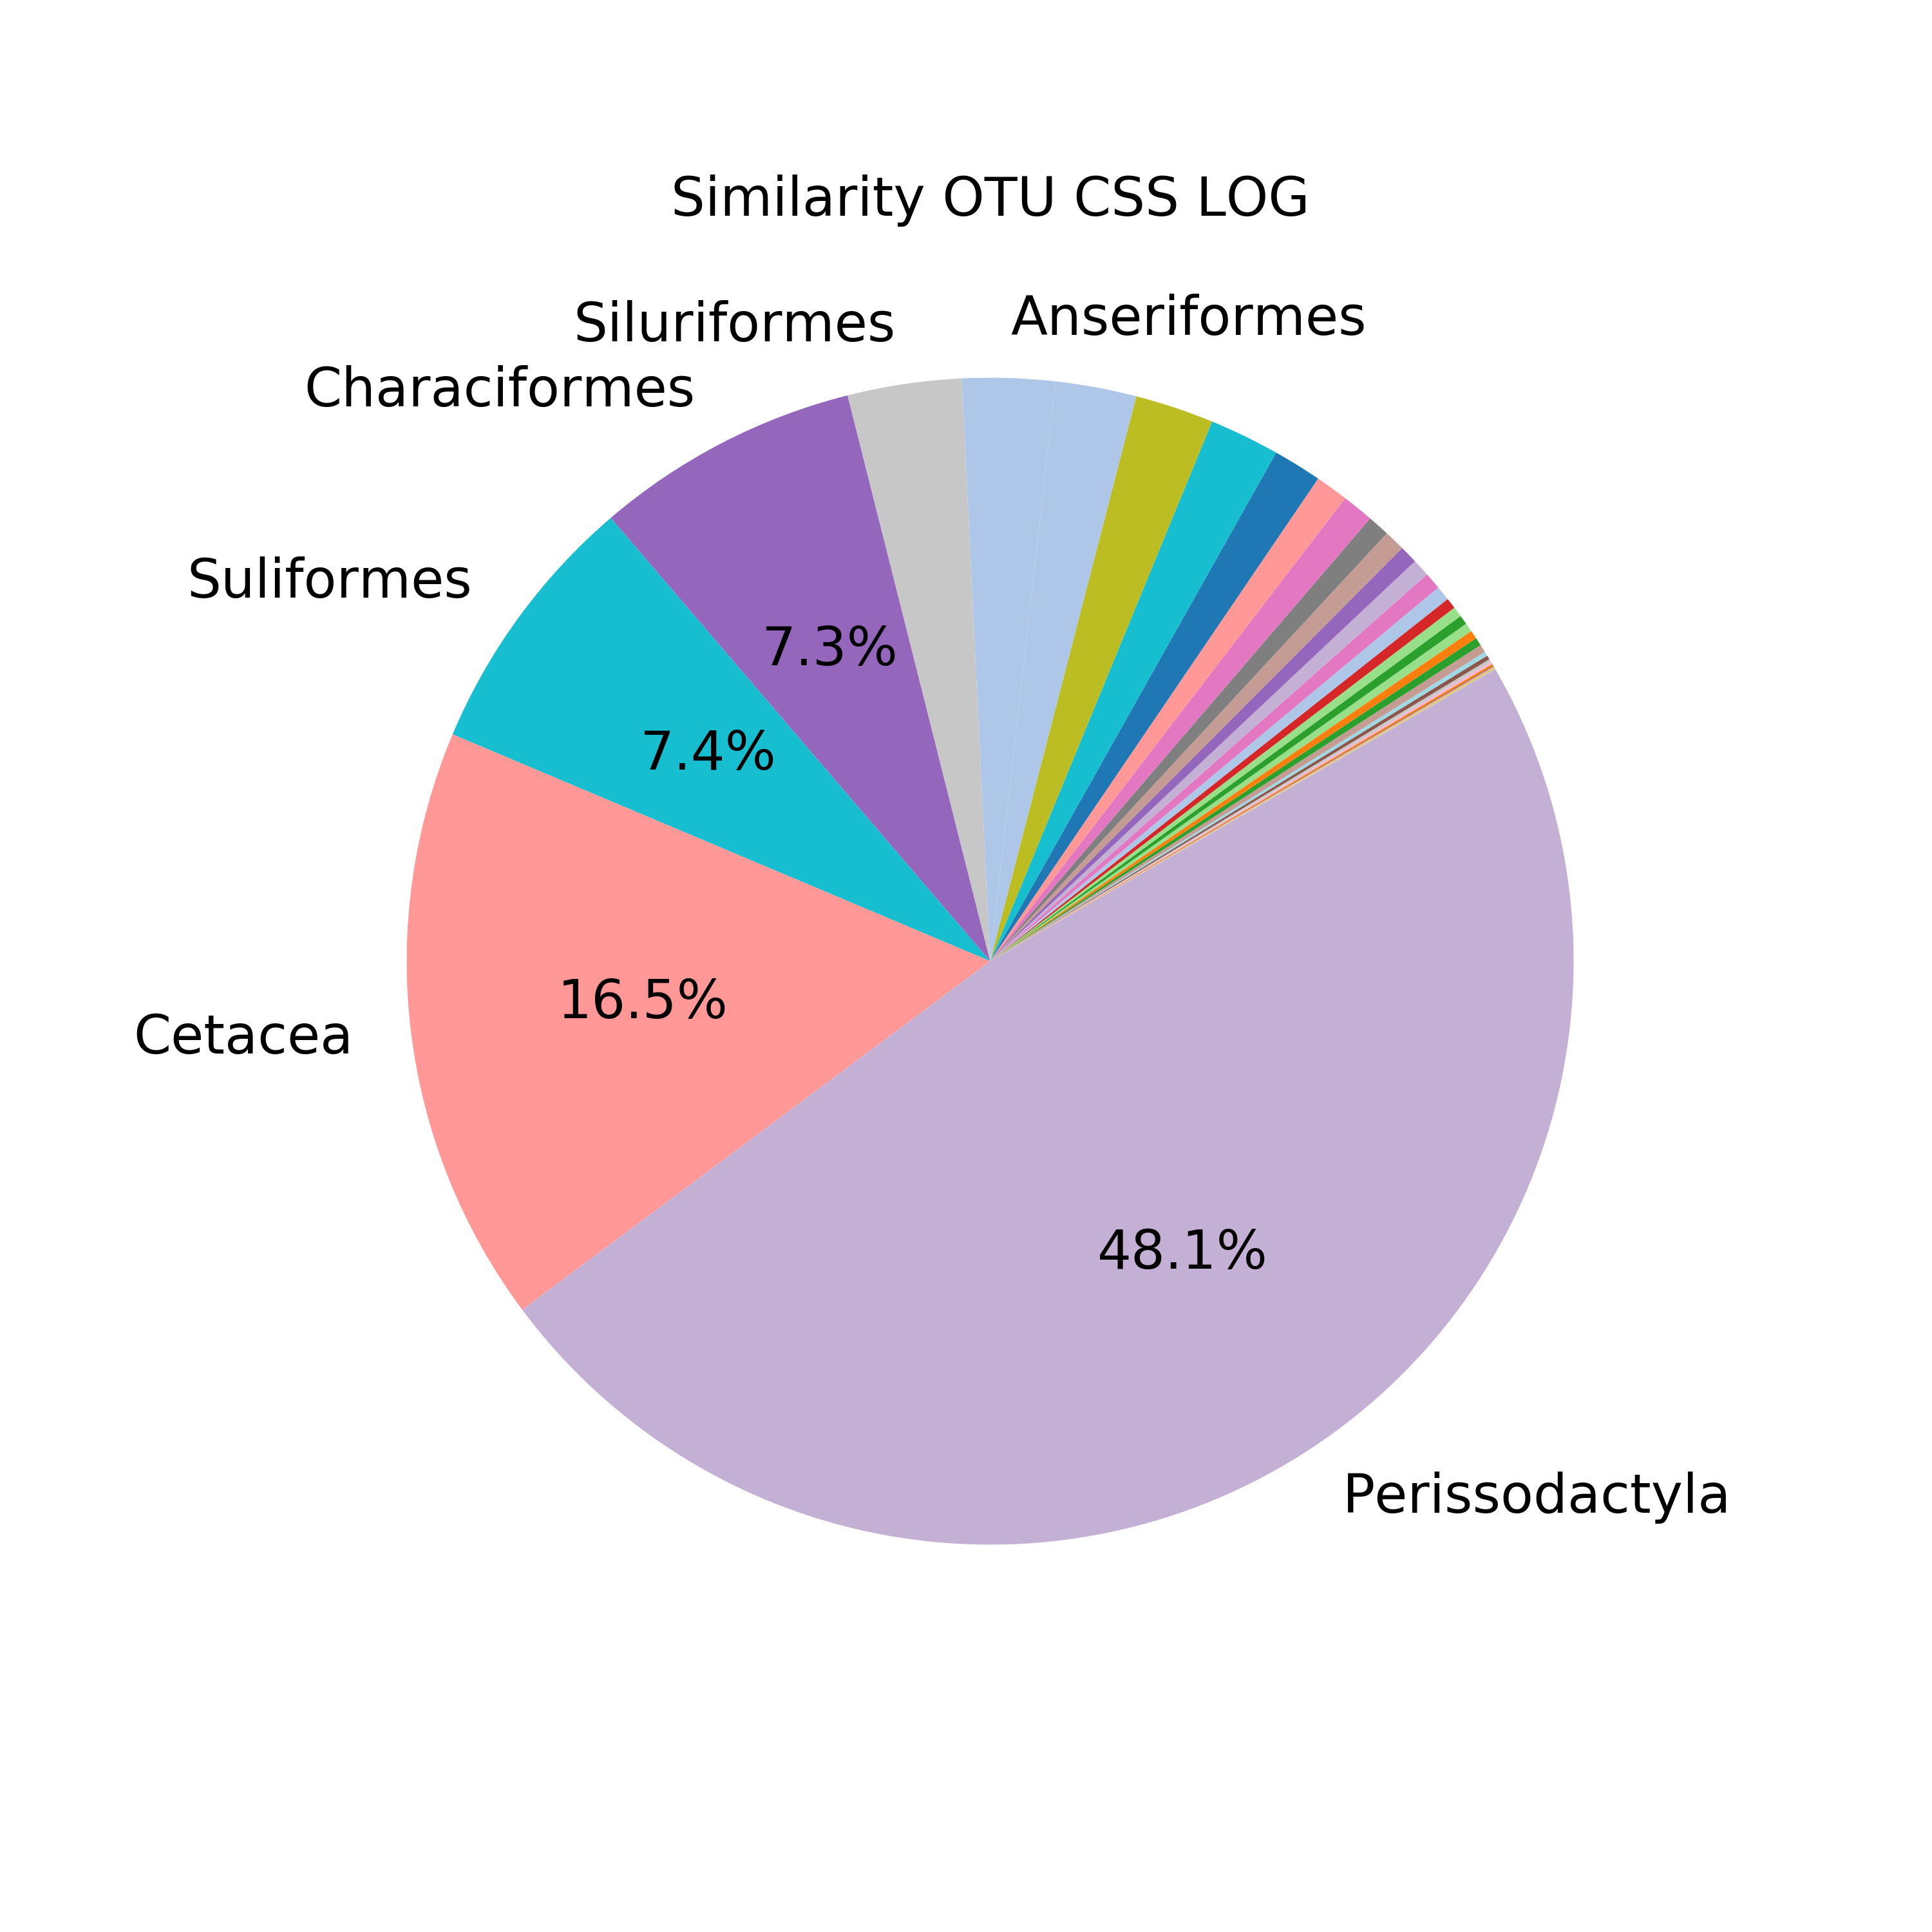
\includegraphics[width=\textwidth]{rfr_sim_mean_pieOTU CSS LOG}
		\caption{}
		\label{fig:simmeanotucsslog}
	\end{subfigure}\\
	\begin{subfigure}{0.45\textwidth}
	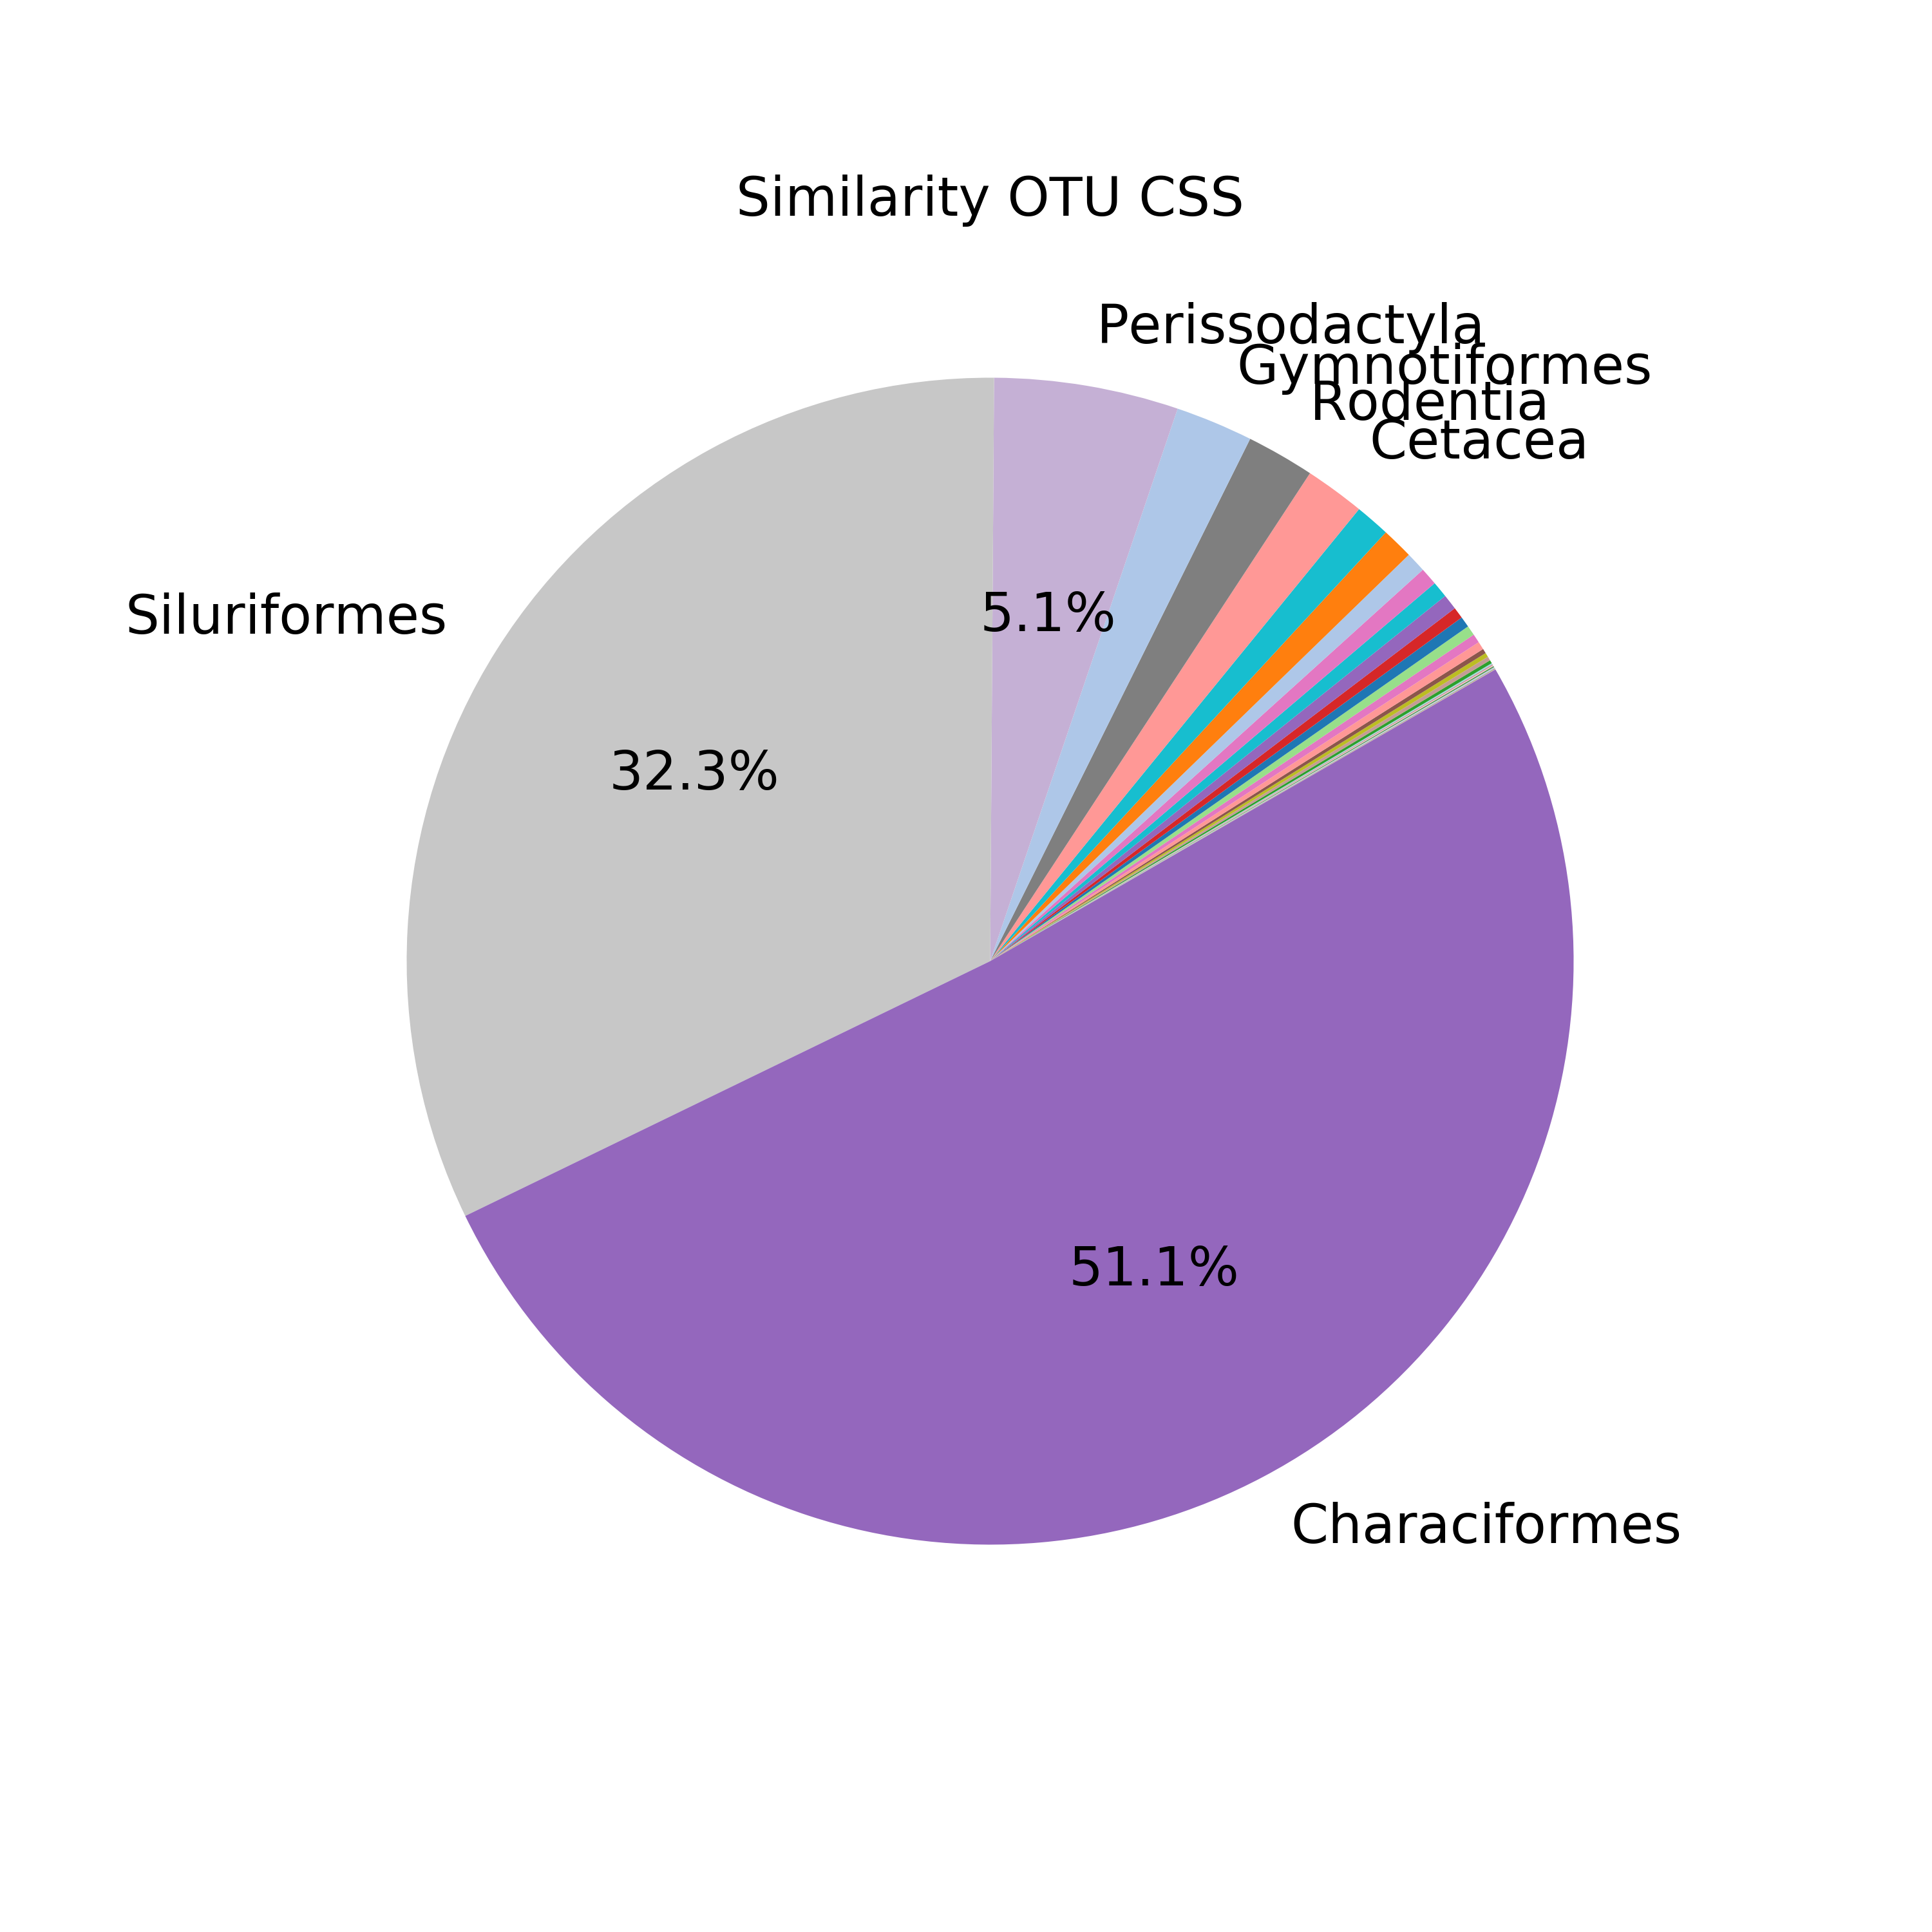
\includegraphics[width=\textwidth]{rfr_sim_sum_pieOTU CSS}
	\caption{}
	\label{fig:simsumotucss}
	\end{subfigure}
	\begin{subfigure}{0.45\textwidth}
	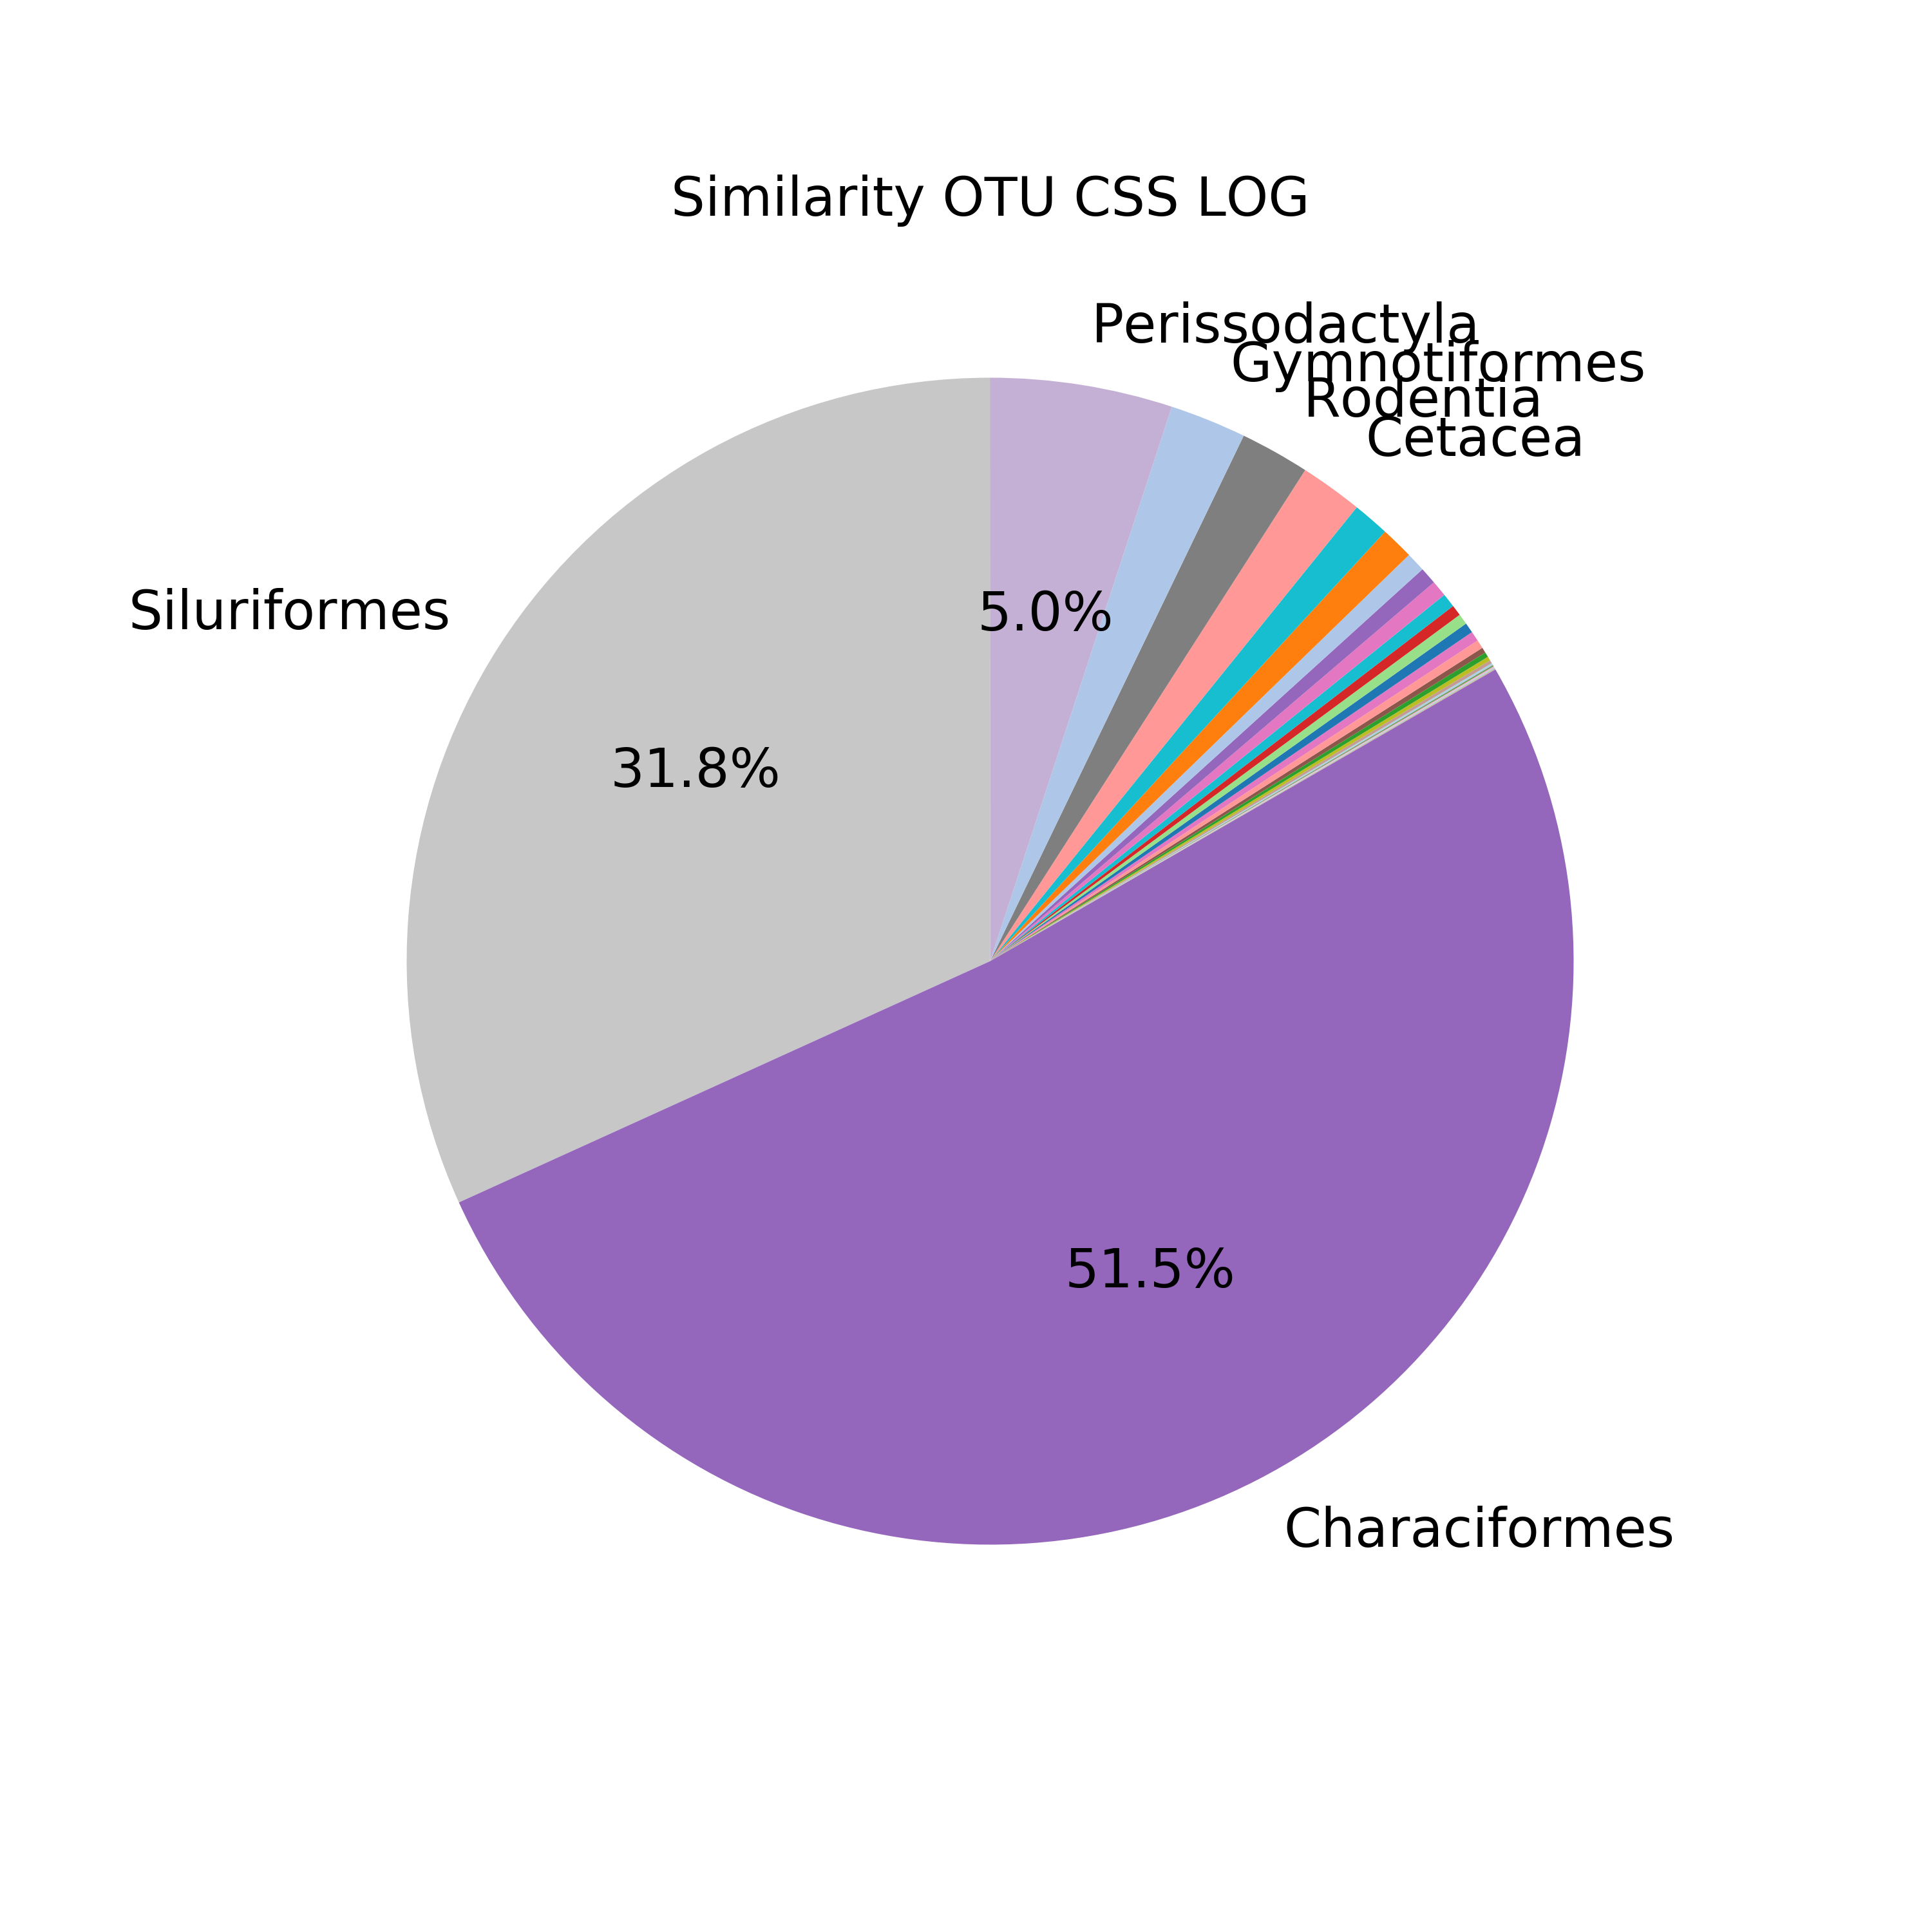
\includegraphics[width=\textwidth]{rfr_sim_sum_pieOTU CSS LOG}
	\caption{}
	\label{fig:simsumotucsslog}
	\end{subfigure}

		\caption{The importance of species per taxonomic order as calculated by Random Forest in the maximum similarity test. Averaging the importance for the sets: OTU CSS \ref{fig:simotucss}, and OTU CSS LOG \ref{fig:simotucsslog}. Summing the importance for the sets: OTU CSS \ref{fig:simsumotucss}, and OTU CSS LOG \ref{fig:simsumotucsslog}. }
	\label{fig:simpie}
\end{figure}

Conclusions can be drawn despite the seemingly contradictory representations of the two methods. This is because all four important Orders are in the top 6 in both methods, and when combined they amount for a substantial part of explanatory power (more than 70\%).    


% DISSIMILARITY
\section{Maximum Dissimilarity}

The classifiers' performance in a maximum dissimilarity setting is worse than that of maximum similarity. The results are summarised in tables \ref{table:lrdissimilarity} and \ref{table:rfrdissimilarity} for Logistic regression and Random Forests respectively. In this setting, Random forests have on average a higher accuracy score. The highest is obtained with OTU MIN CSS (90.45\%), but OTU CSS and OTU CSS LOG come close (90.24\%). Logistic regression has the highest accuracy with PCoA CSS and OTU CSS LOG (87.80\%), and with PCoA coming close (86.58\%).

Again, the $L_1$ penalty reduced many coefficients to zero; among the best performing sets, PCoA CSS 88.33\%   
% Logistic Dissimilarity
\begin{table}[h]
	\centering
	\begin{tabular}{l c  c c}
		\toprule
		&\multicolumn{2}{c}{Confusion Matrix} & Accuracy\\
		Features used & Predicted Black&Predicted White&\\
		\midrule
		\multirow{2}{*}{OTU} &5 &16&\multirow{2}{*}{79.27\%}\\
		&	 18&125&\\
		\cmidrule{2-3}
		\multirow{2}{*}{OTU LOW} &5 &16&\multirow{2}{*}{79.88\%}\\
		&	 17&126&\\
		\cmidrule{2-3}
		\multirow{2}{*}{OTU CSS}&7 &14&\multirow{2}{*}{82.93\%}\\
		&	 14&129&\\
		\cmidrule{2-3}
		\multirow{2}{*}{OTU Min CSS}&3 &18&\multirow{2}{*}{79.61\%}\\
		&	 14&122&\\
		\cmidrule{2-3}
		\multirow{2}{*}{OTU CSS LOG}&5 &16&\multirow{2}{*}{87.80\%}\\
		&	 4&139&\\
		\cmidrule{2-3}
		\multirow{2}{*}{PCoA Bray-Curtis} &7 &14&\multirow{2}{*}{86.59\%}\\
		&	 8&135&\\
		\cmidrule{2-3}
		\multirow{2}{*}{PCoA Bray-Curtis CSS} &9 &12&\multirow{2}{*}{87.80\%}\\
		&	 8&135&\\
		\bottomrule
	\end{tabular}
	\caption{Results from maximising dissimilarity using Logistic Regression}
	\label{table:lrdissimilarity}
\end{table}



% RFR dissimilarity table
\begin{table}[h]
	\centering
	\begin{tabular}{l c  c c}
		\toprule
		&\multicolumn{2}{c}{Confusion Matrix} & Accuracy\\
		Features used & Predicted Black&Predicted White&\\
		\midrule
		\multirow{2}{*}{OTU} &4 &17&\multirow{2}{*}{83.50\%}\\
		&	 10&133&\\
		\cmidrule{2-3}
		\multirow{2}{*}{OTU LOW} &2&19&\multirow{2}{*}{82.32\%}\\
		&	 10&133&\\
		\cmidrule{2-3}
		\multirow{2}{*}{OTU CSS}&7 &14&\multirow{2}{*}{90.24\%}\\
		&	 2&141&\\
		\cmidrule{2-3}
		\multirow{2}{*}{OTU Min CSS}&7 &14&\multirow{2}{*}{90.45\%}\\
		&	 1&135&\\
		\cmidrule{2-3}
		\multirow{2}{*}{OTU CSS LOG}&7 &14&\multirow{2}{*}{90.24\%}\\
		&	 2&141&\\
		\cmidrule{2-3}
		\multirow{2}{*}{PCoA Bray-Curtis} &0 &21&\multirow{2}{*}{86.59\%}\\
		&	 1&142&\\
		\cmidrule{2-3}
		\multirow{2}{*}{PCoA Bray-Curtis CSS} &0 &21&\multirow{2}{*}{84.15\%}\\
		&	 5&138&\\
		\bottomrule
	\end{tabular}
	\caption{Results from maximising dissimilarity using Random Forest}
	\label{table:rfrdissimilarity}
\end{table}


%%DISIMILARITY PIE CHART
\begin{figure}[h]
	\centering
	\begin{subfigure}{0.45\textwidth}
		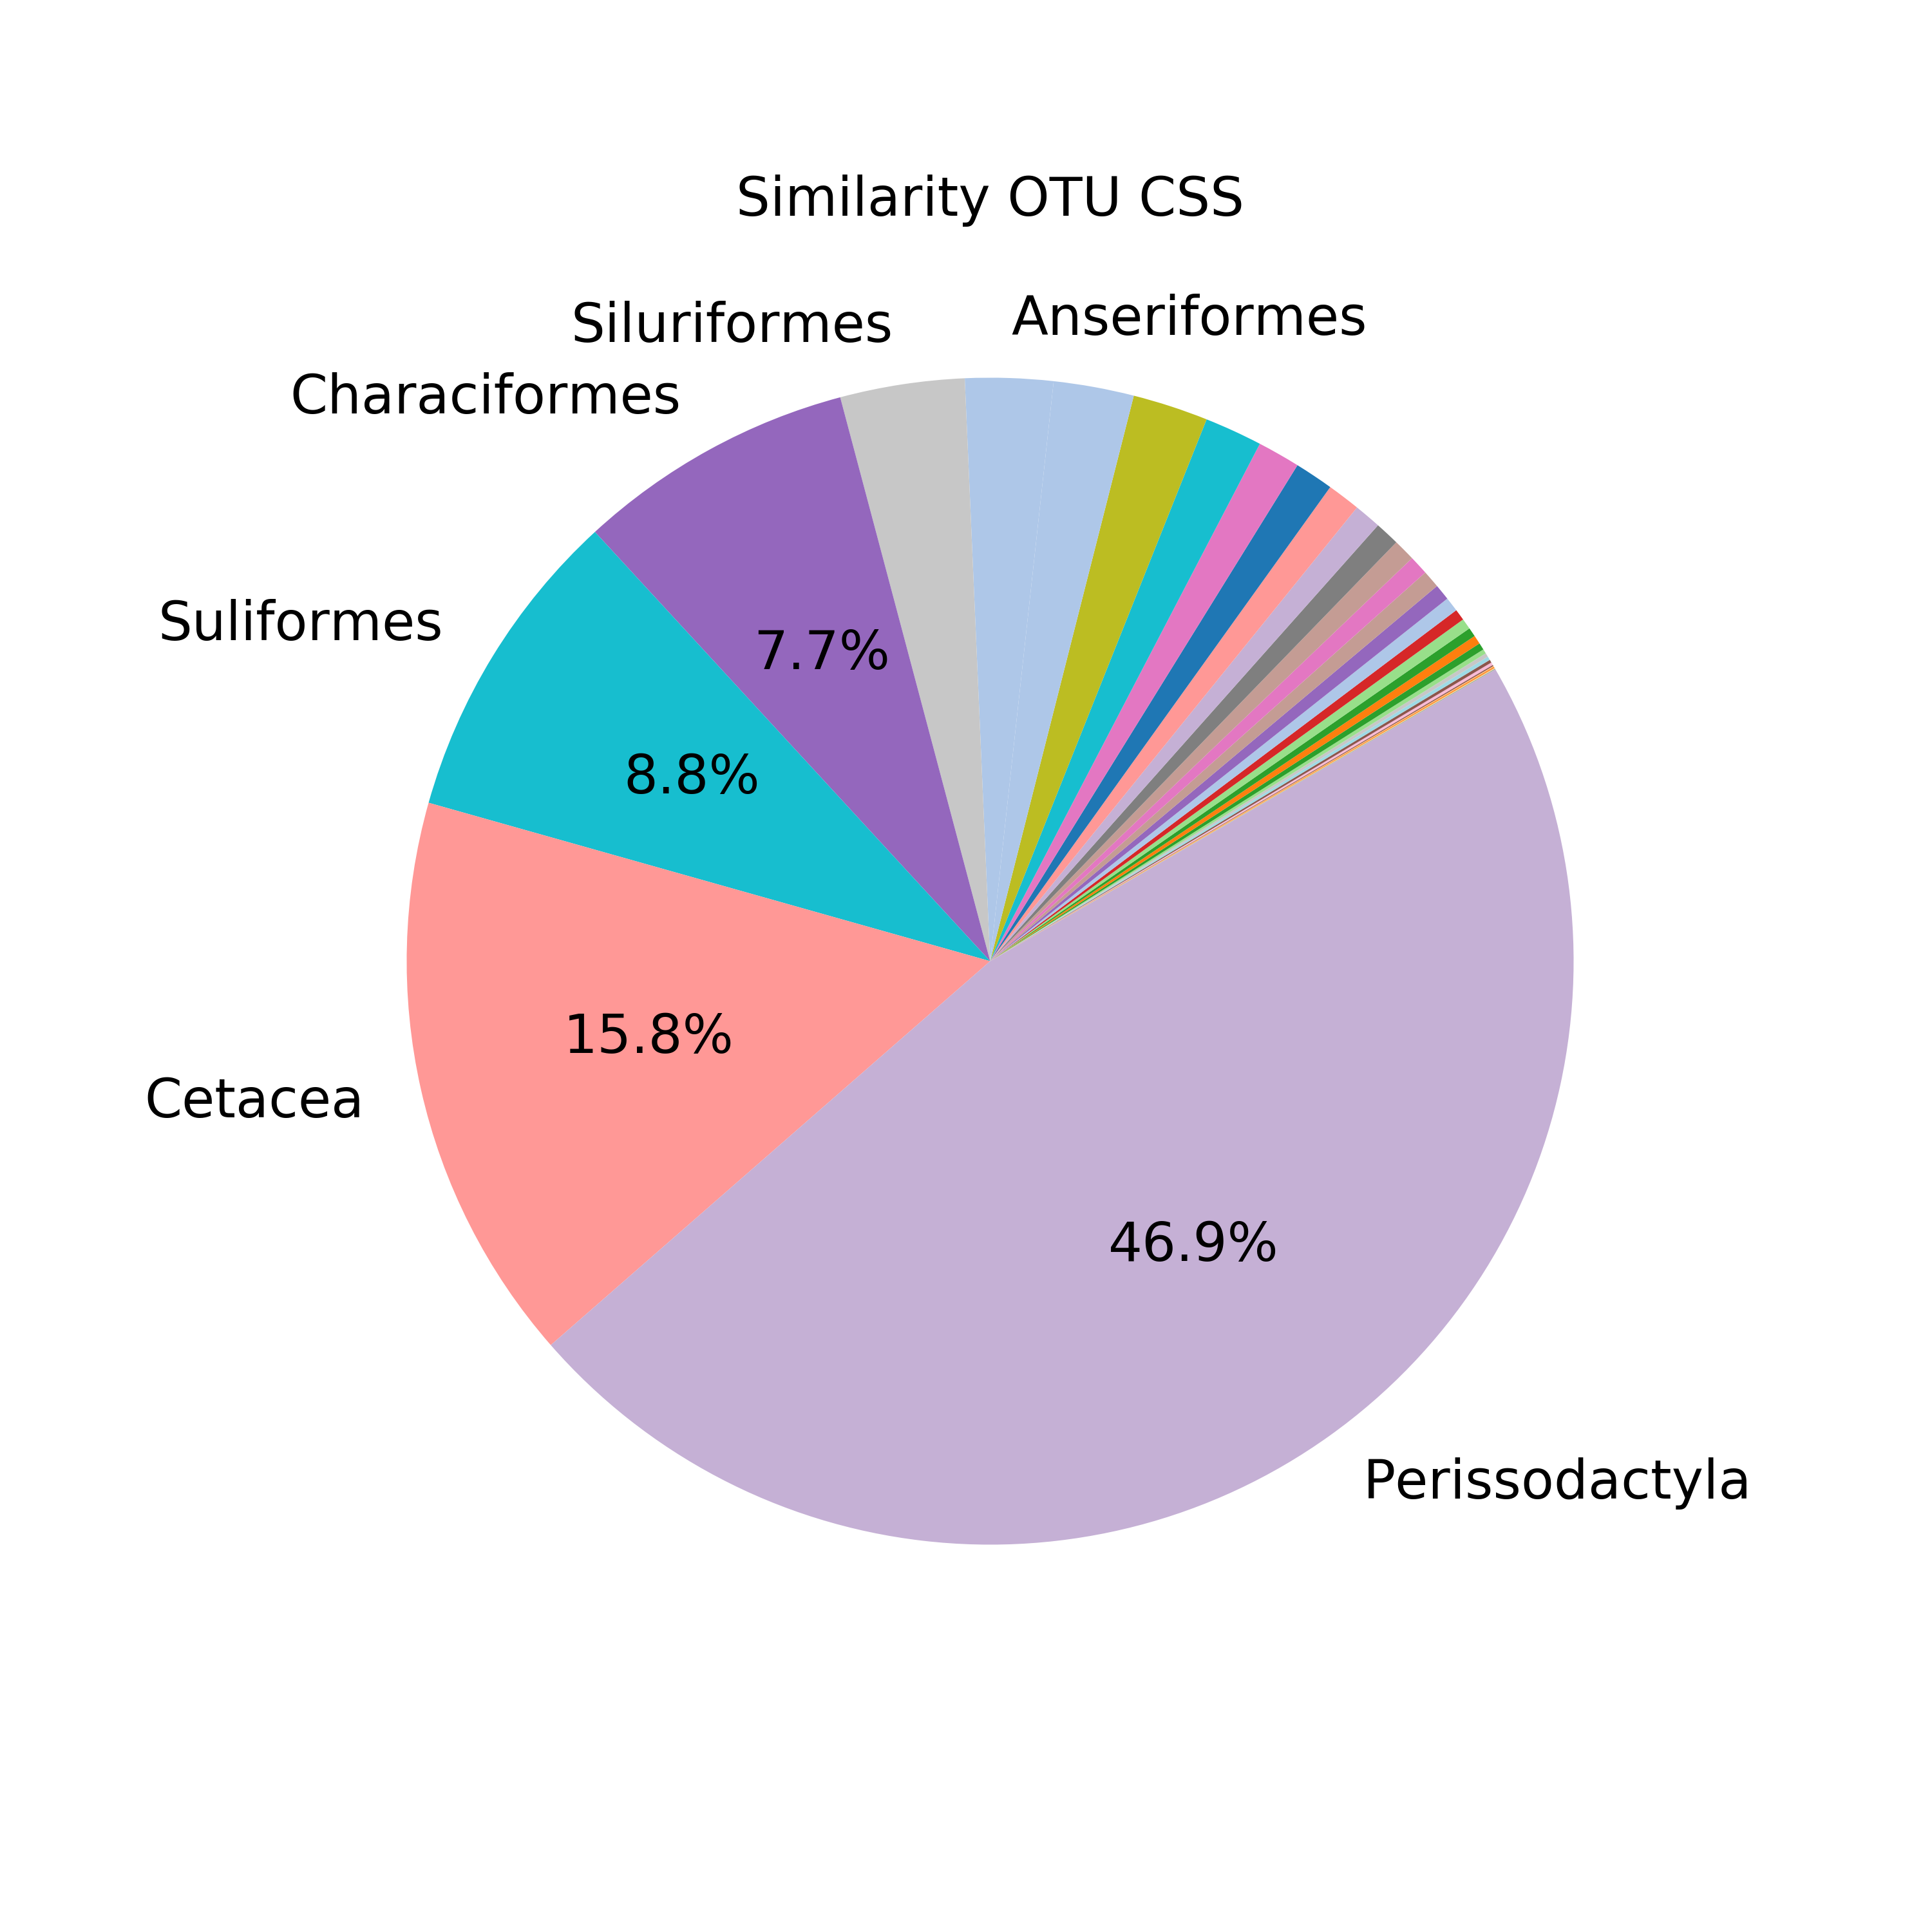
\includegraphics[width=\textwidth]{rfr_dis_mean_pieOTU CSS}
		\caption{}
		\label{fig:dissimotucss}
	\end{subfigure}
	\begin{subfigure}{0.45\textwidth}
		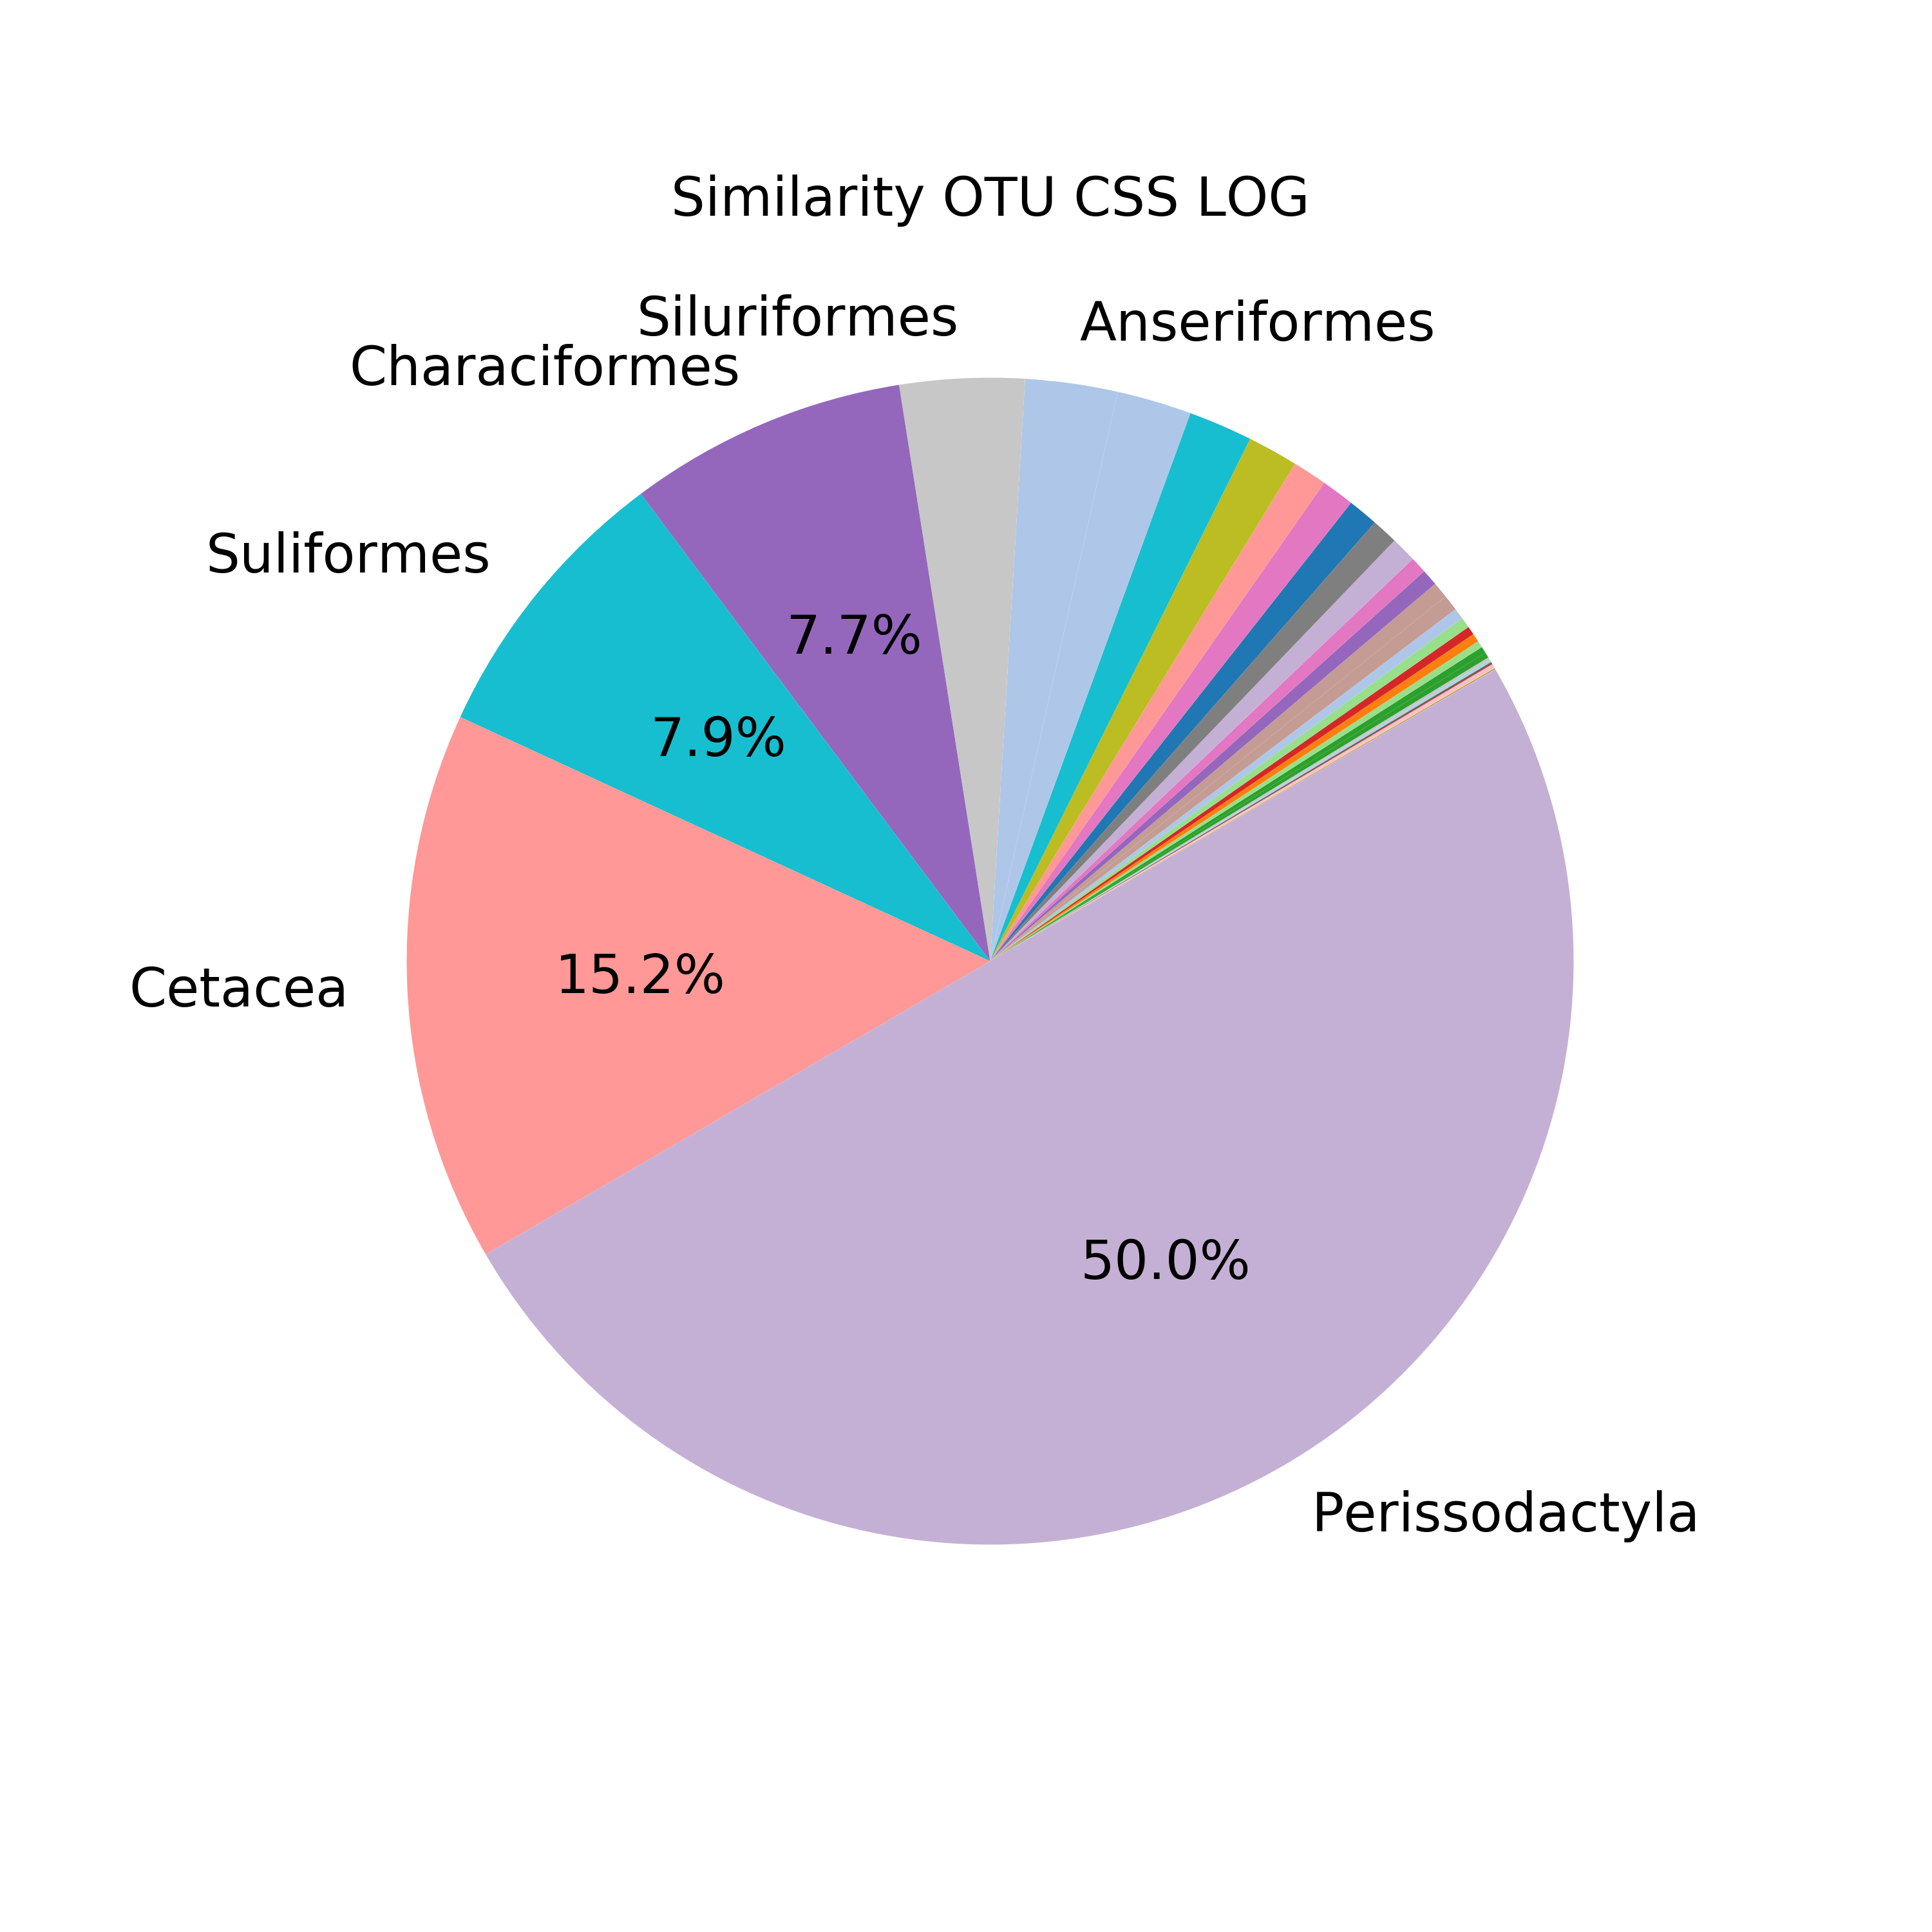
\includegraphics[width=\textwidth]{rfr_dis_mean_pieOTU CSS LOG}
		\caption{}
		\label{fig:dissimotucsslog}
	\end{subfigure}\\
		\begin{subfigure}{0.45\textwidth}
		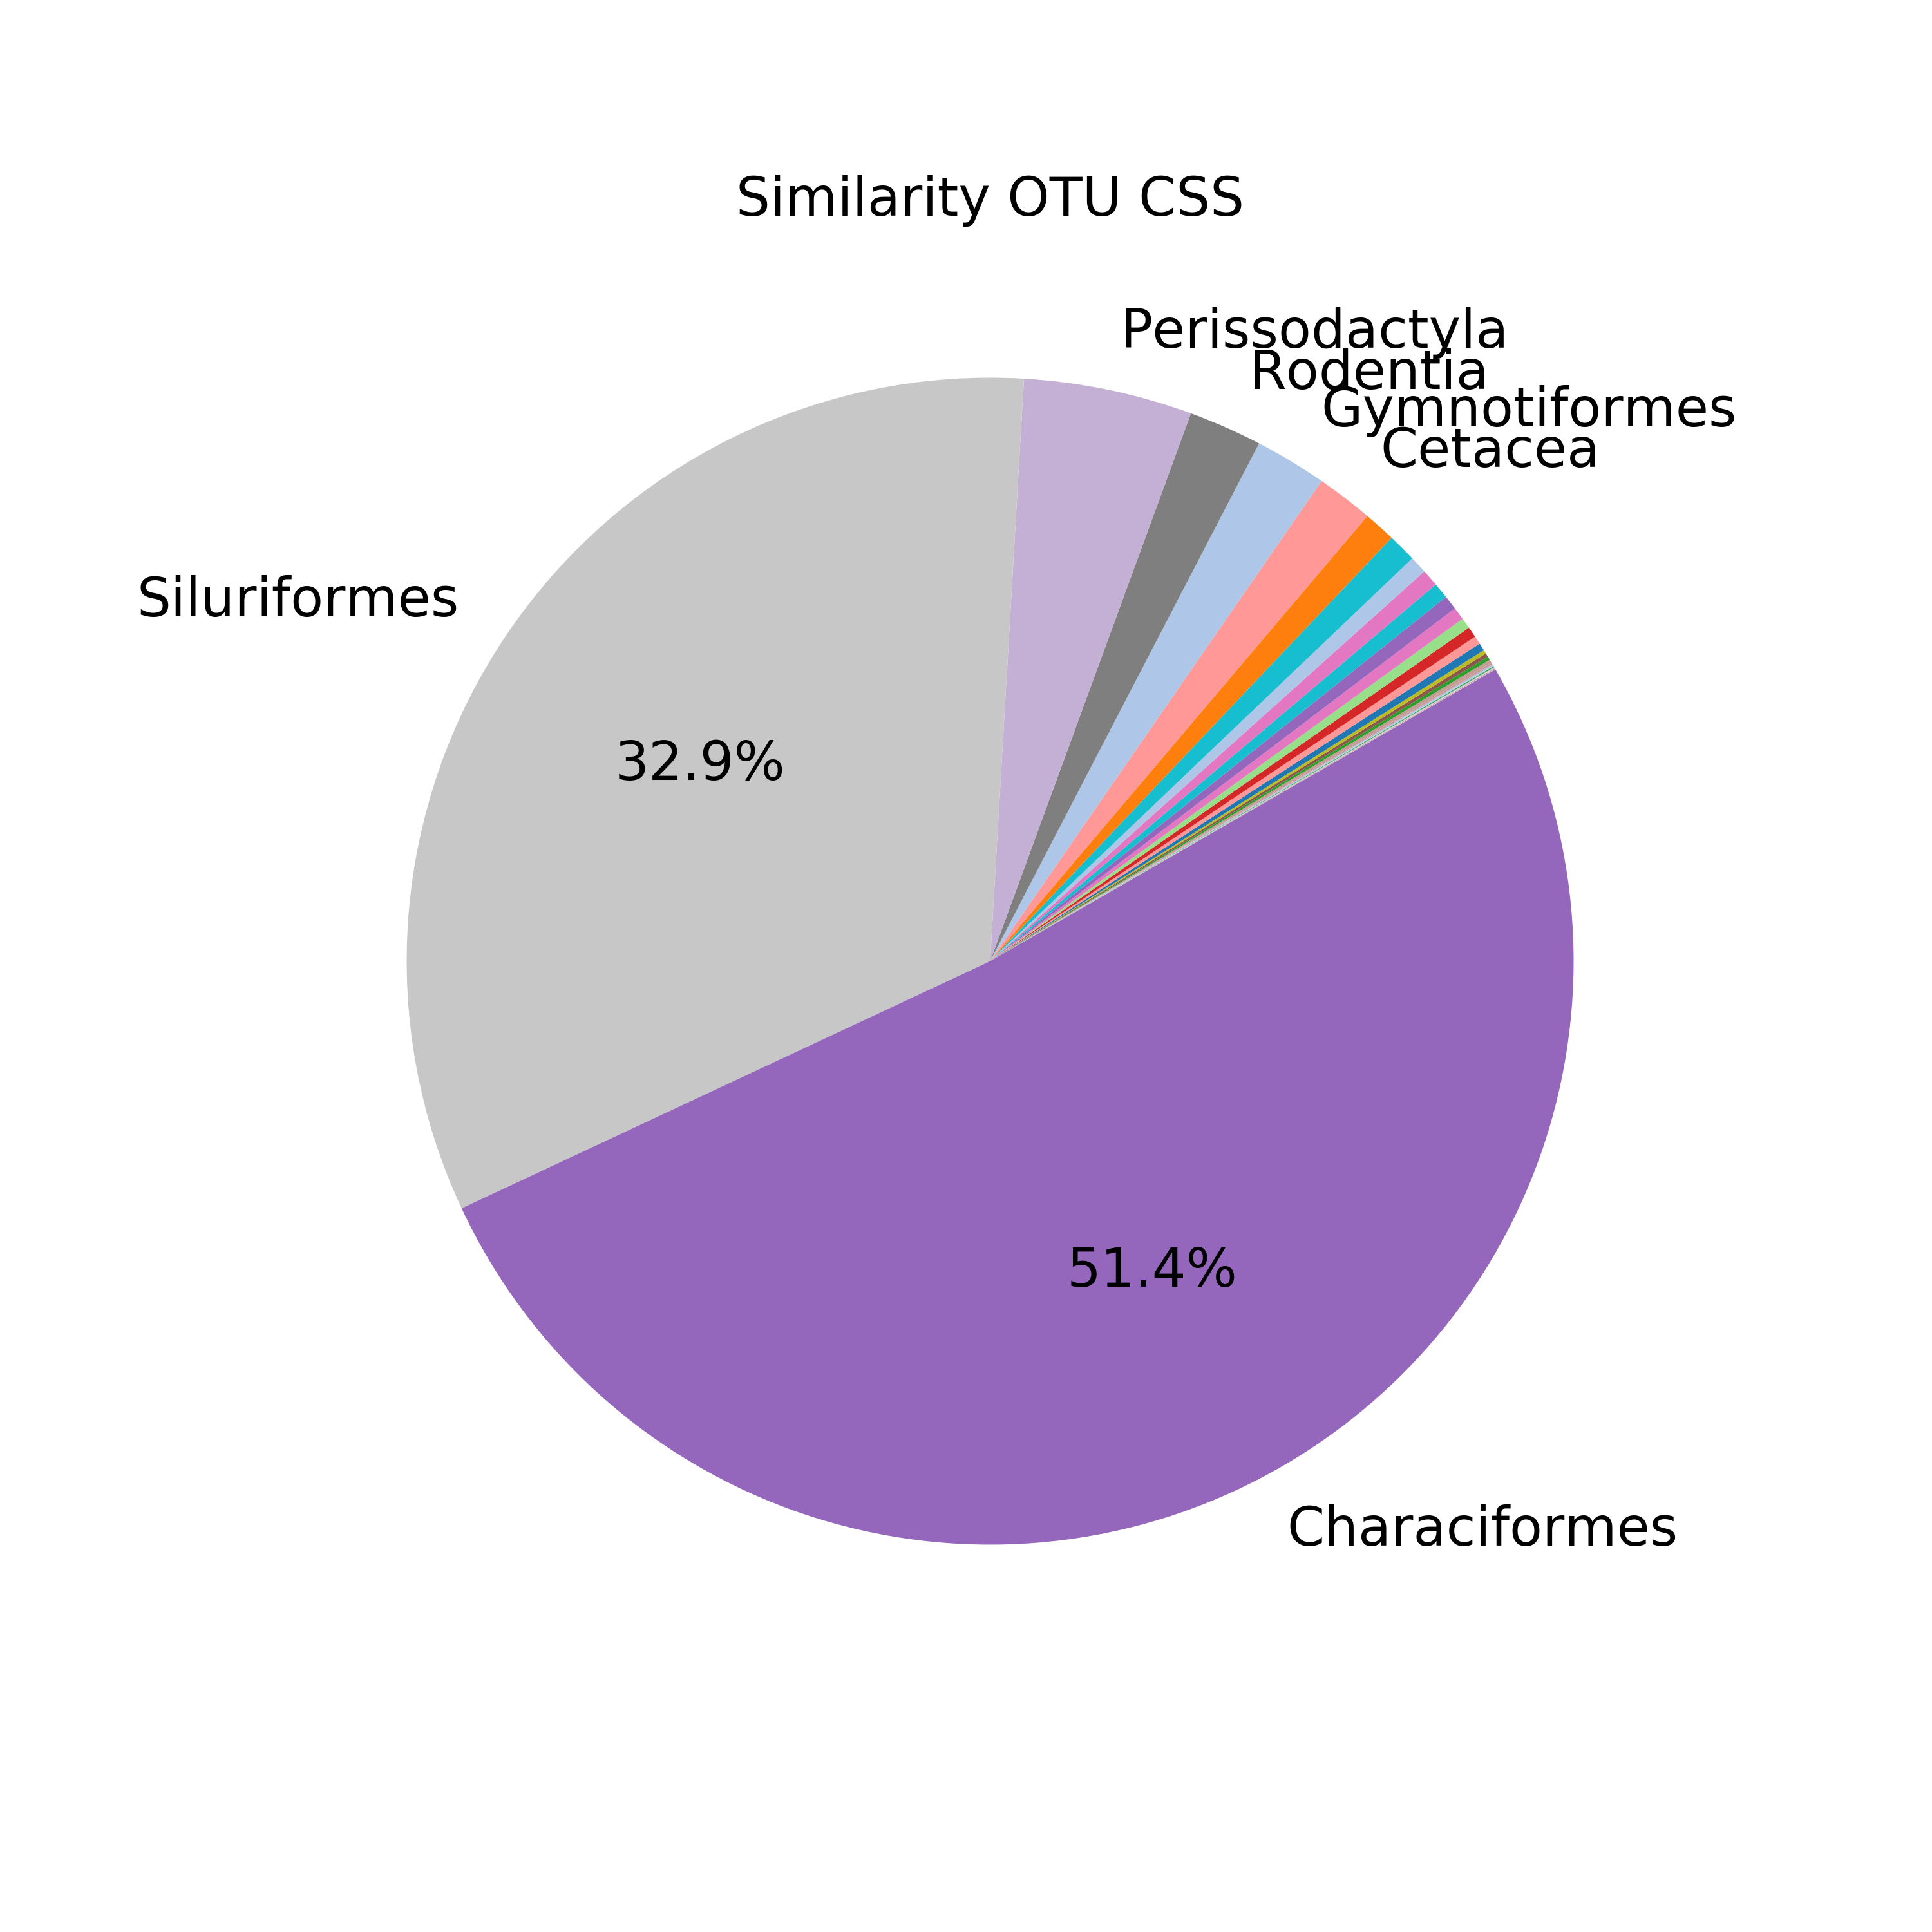
\includegraphics[width=\textwidth]{rfr_dis_sum_pieOTU CSS}
		\caption{}
		\label{fig:dissimotucss}
	\end{subfigure}
	\begin{subfigure}{0.45\textwidth}
	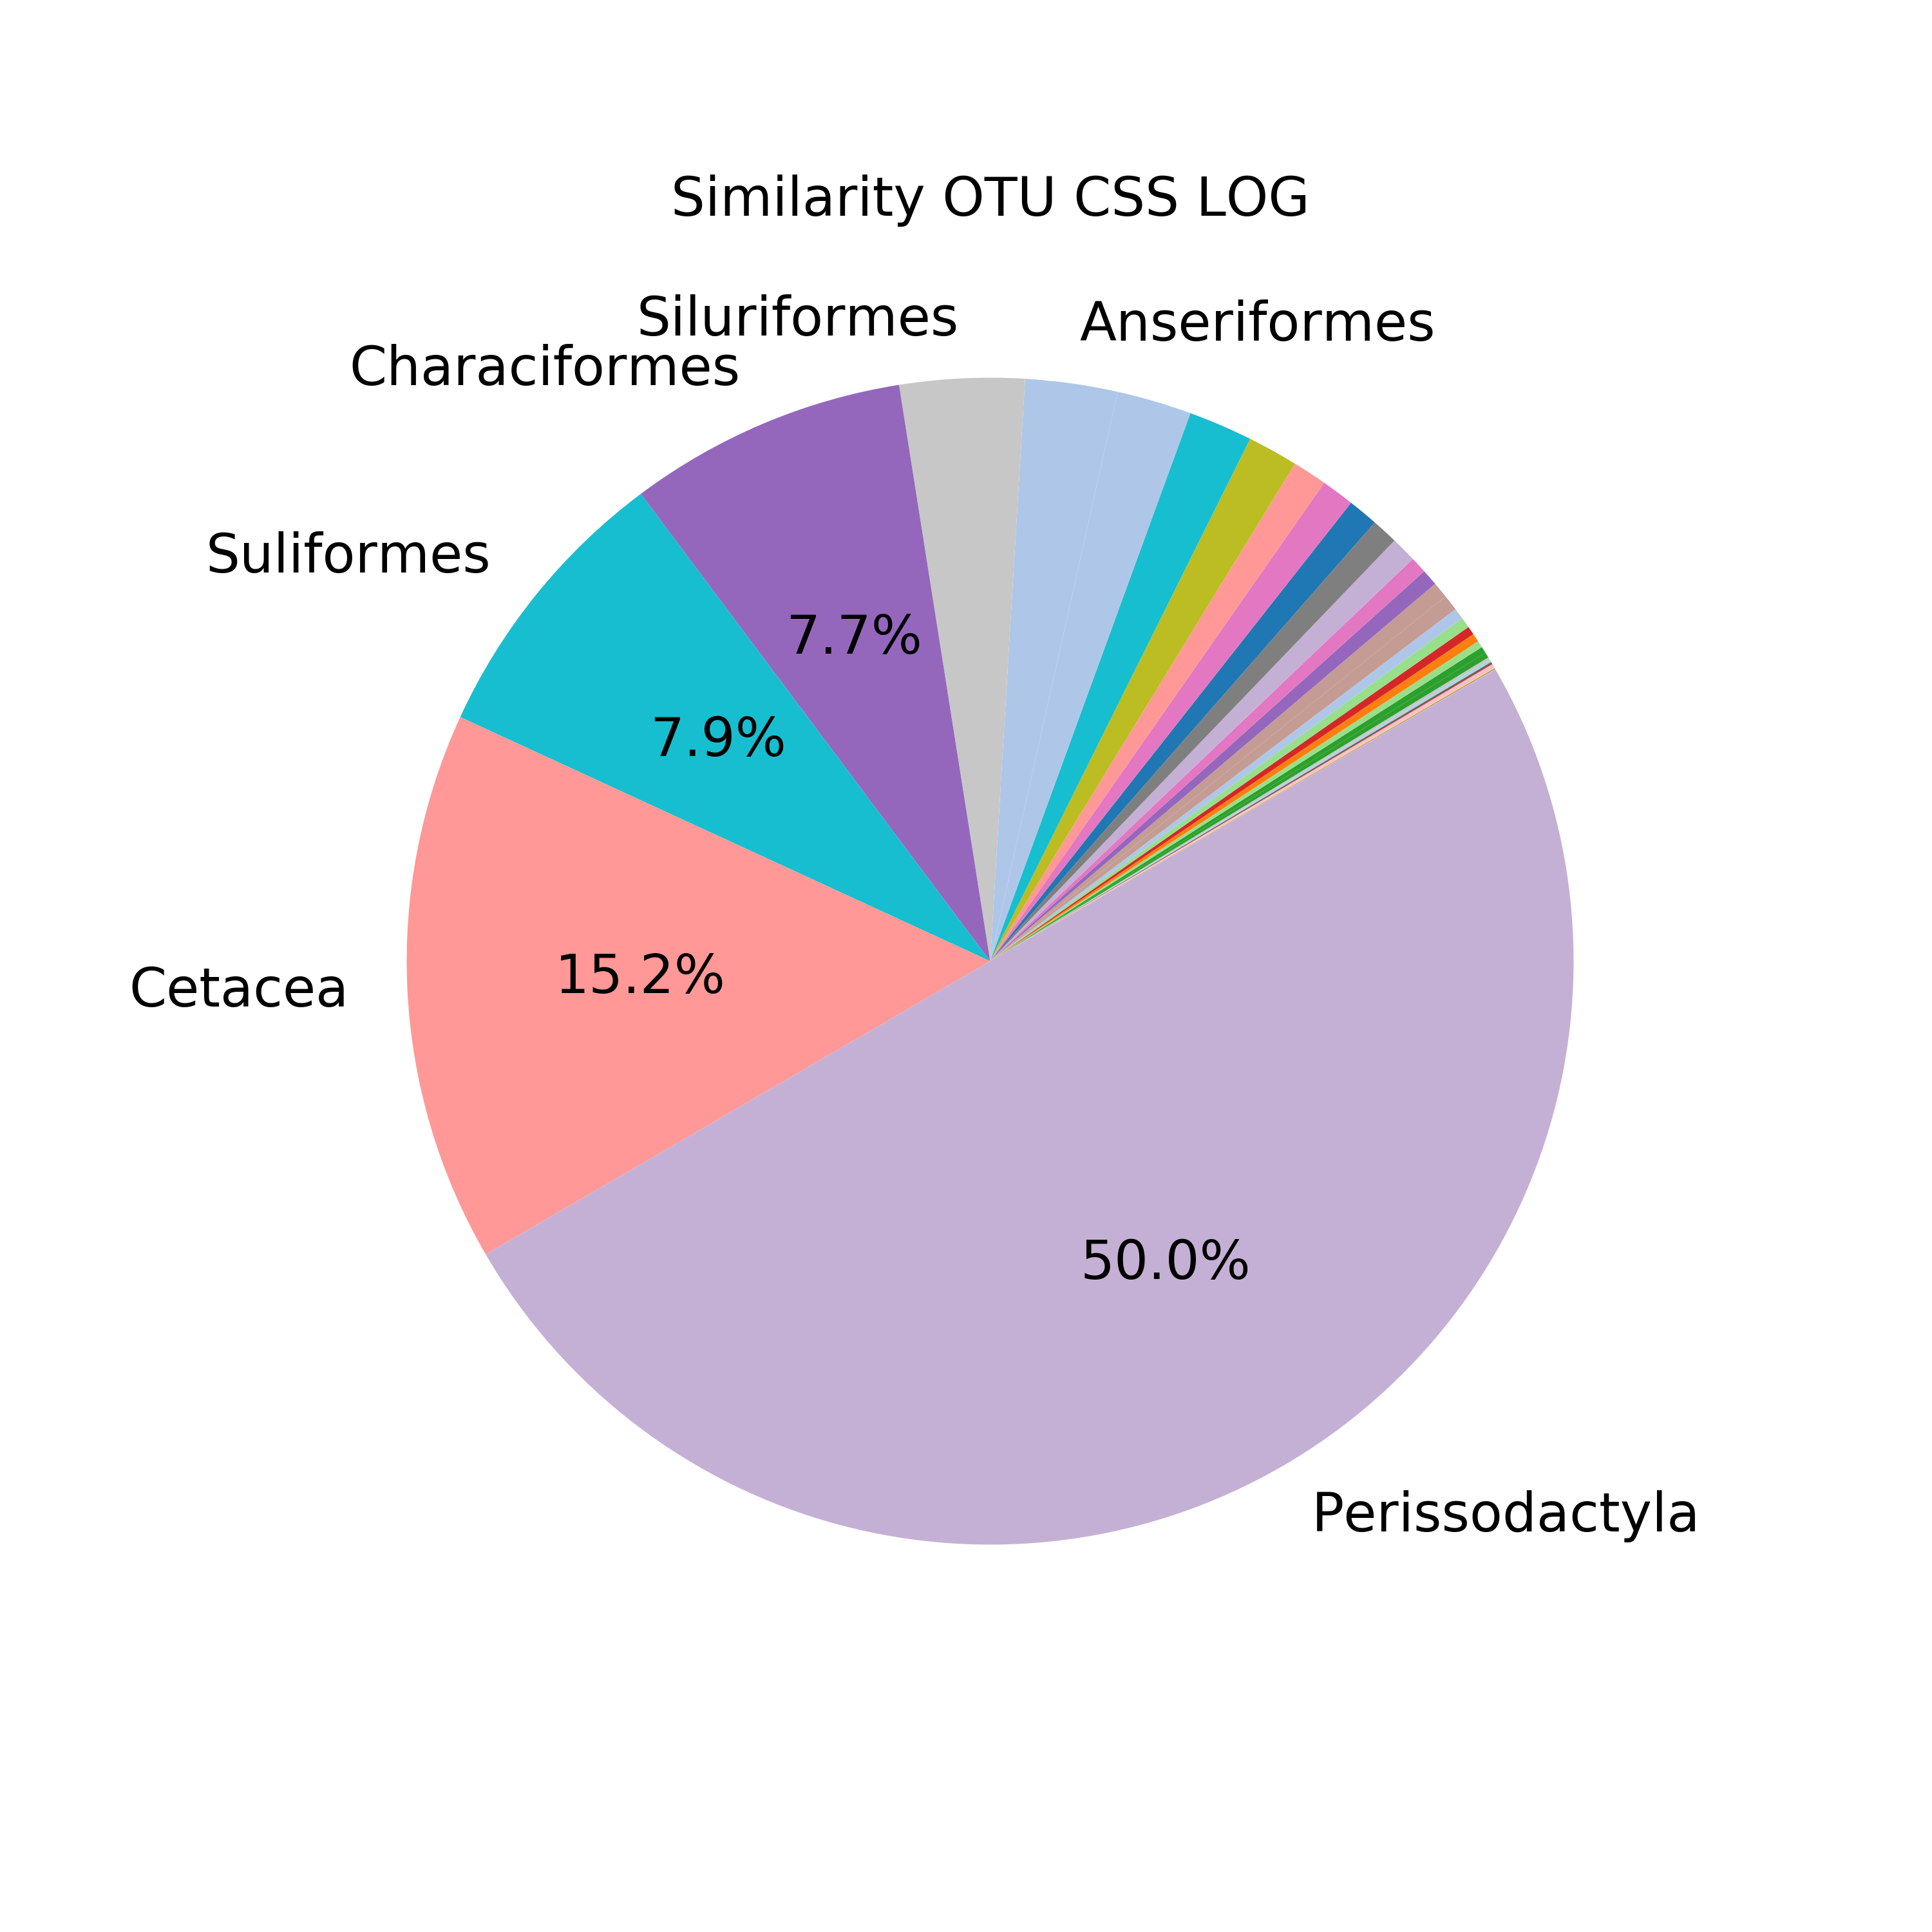
\includegraphics[width=\textwidth]{rfr_dis_sum_pieOTU CSS LOG}
	\caption{}
	\label{fig:dissimotucsslog}
\end{subfigure}\\

	\caption{The average importance of species per taxonomic order as calculated by Random Forest in the maximum dissimilarity test on OTU \ref{fig:dissimotu}, OTU CSS \ref{fig:dissimotucss}, OTU Min CSS \ref{fig:dissimotumincss}, and OTU CSS LOG \ref{fig:dissimotucsslog}.  }
	\label{fig:dispie}
\end{figure}


